\documentclass[paper=a4, fontsize=10pt]{jlreq}

\usepackage{amsmath, amssymb}
\usepackage{enumerate}
\usepackage{tikz}
\usepackage{listings, xcolor}
\usepackage{graphicx}

\lstset{
  basicstyle = {\ttfamily},
  frame = {tbrl},
  breaklines = true,
  numbers = left,
  showspaces = false,
  showstringspaces = false,
  showtabs = false,
  keywordstyle = \color{blue},
  identifierstyle = \color{black},
  stringstyle = \color{brown},
  captionpos = t
}

\title{生体情報計測による視線のカスケード現象と負荷増大に伴う筋活動量の検証}
\author{学籍番号 1280391 \\ 細川 夏風}
\date{\today}

\begin{document}

\maketitle

\section{眼球運動計測実験}
\subsection{顔画像の魅力度判断における視線のカスケード現象の検証}
\subsubsection{目的}
顔の魅力度を判断する際，最終的に選択する対象を決定する直前に，その対象に対する注視時間や確率が増加する「視線のカスケード現象」が存在する\cite{bsd_eyemovement, tane_michimata}．本実験では，左右に提示された顔画像から魅力的な方を選択する課題を行い，選択行動と眼球運動の関連性が実際に確認されるかを検証することを目的とする．

\subsubsection{方法}
実験参加者は10班の代表者1名とした．時間解像度の高い眼球運動計測装置としてEye Link II（SR Research社）を使用し，刺激提示用の装置としてPCおよび液晶ディスプレイを用いた．

まず，参加者の頭部にEye Link IIのアイカメラを装着し，視線方向のキャリブレーションおよびバリデーションを実施した．次に，ディスプレイの中心に提示される円および十字の固視点を注視させた．その後，2枚の女性の顔画像が画面の左右に同時に提示されるため，参加者には両者をよく見比べ，より魅力的に感じる方を直感的に素早く判断して，キーボード（左を選択する場合は4，右を選択する場合は6）を押して回答させた．この顔画像の提示からキー押しまでの試行を，計20回繰り返して眼球運動データを記録した．

\subsubsection{結果}
眼球運動計測実験の様子を図\ref{fig:eyelink}に，取得された視線データ画面を図\ref{fig:eyelinkdata}に示す．また，顔画像の魅力度判断課題において解析された，選択までの時間と選択する顔に対する注視の確率の推移を図\ref{fig:cascade}に示す．図\ref{fig:cascade}より，選択ボタンを押す約1秒前から，選択する顔画像に対する注視確率が上昇し始める傾向が確認された．

\begin{figure}[htbp]
  \centering
  \begin{minipage}{0.45\columnwidth}
    \centering
    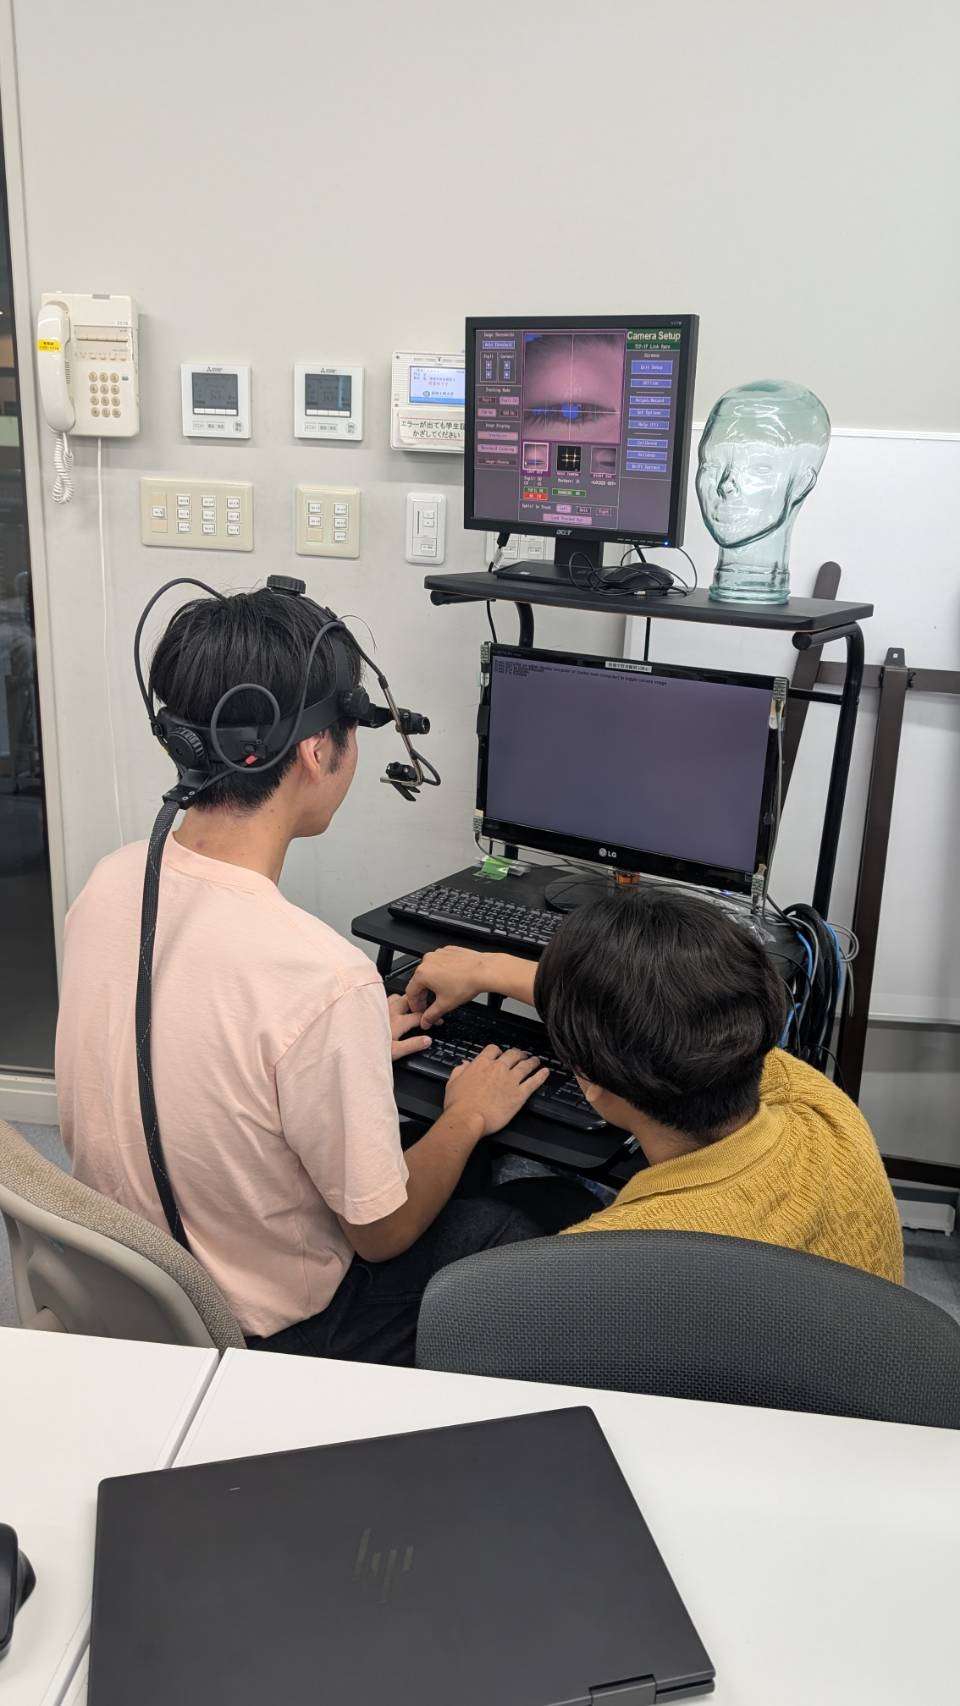
\includegraphics[width=\columnwidth]{eyelink.JPG}
    \caption{眼球運動計測の様子}
    \label{fig:eyelink}
  \end{minipage}
  \hspace{0.04\columnwidth}
  \begin{minipage}{0.45\columnwidth}
    \centering
    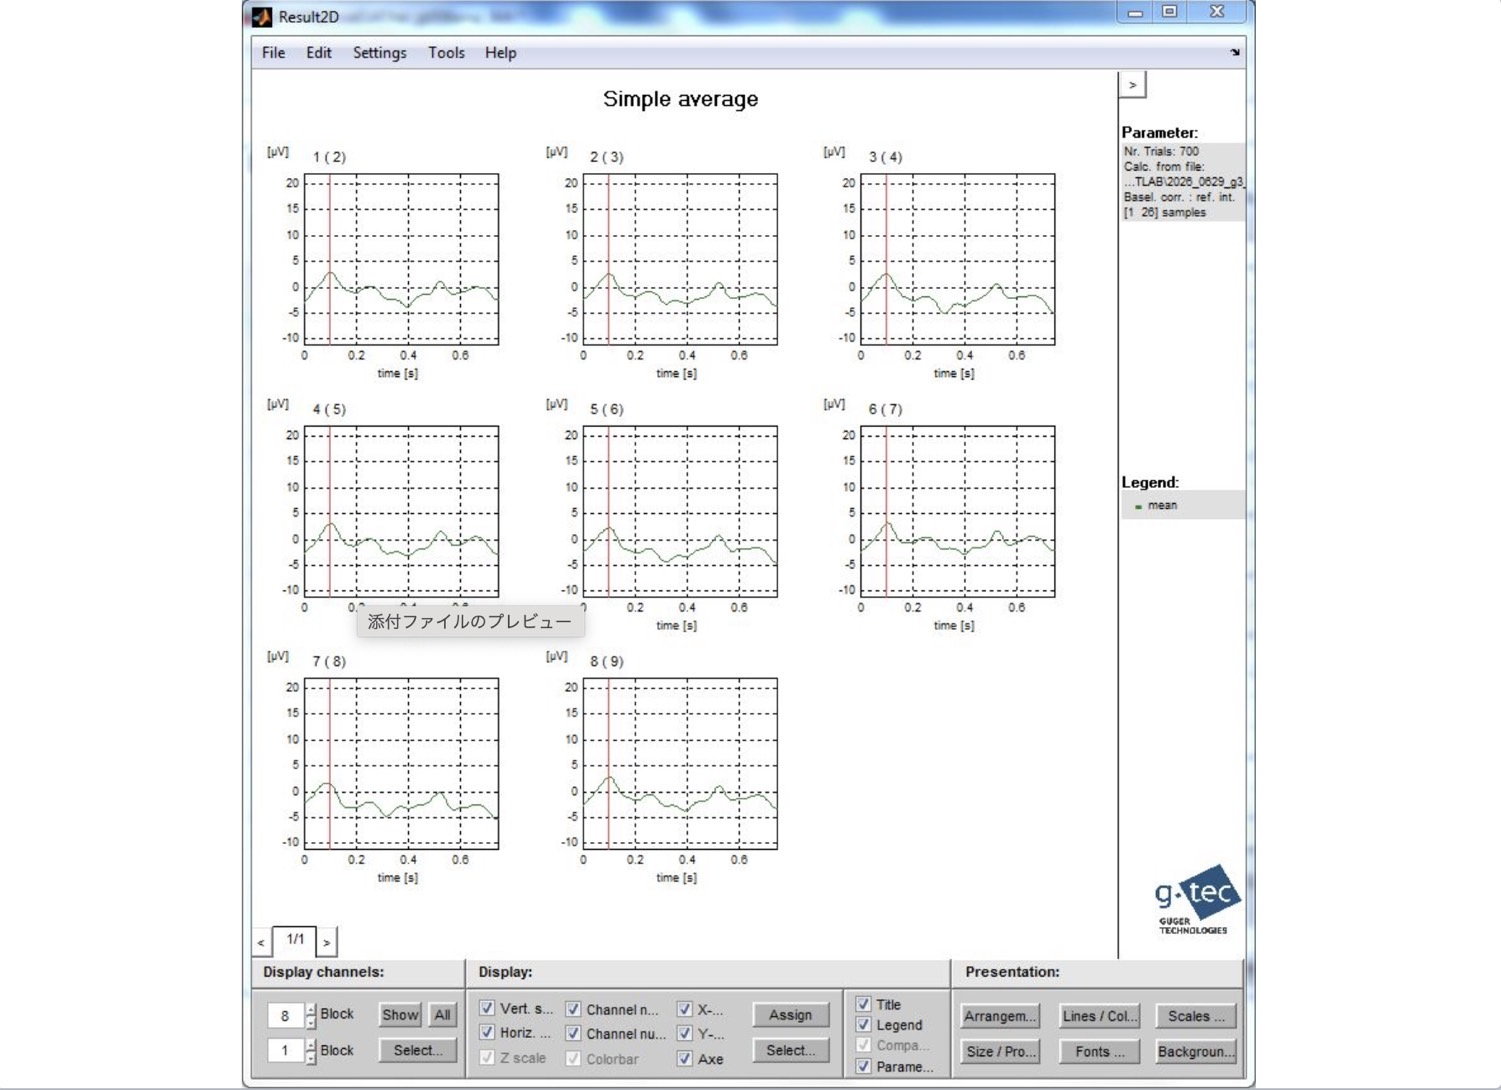
\includegraphics[width=\columnwidth]{eyelinkdata.JPG}
    \caption{取得された視線データ}
    \label{fig:eyelinkdata}
  \end{minipage}
\end{figure}

\begin{figure}[htbp]
  \centering
  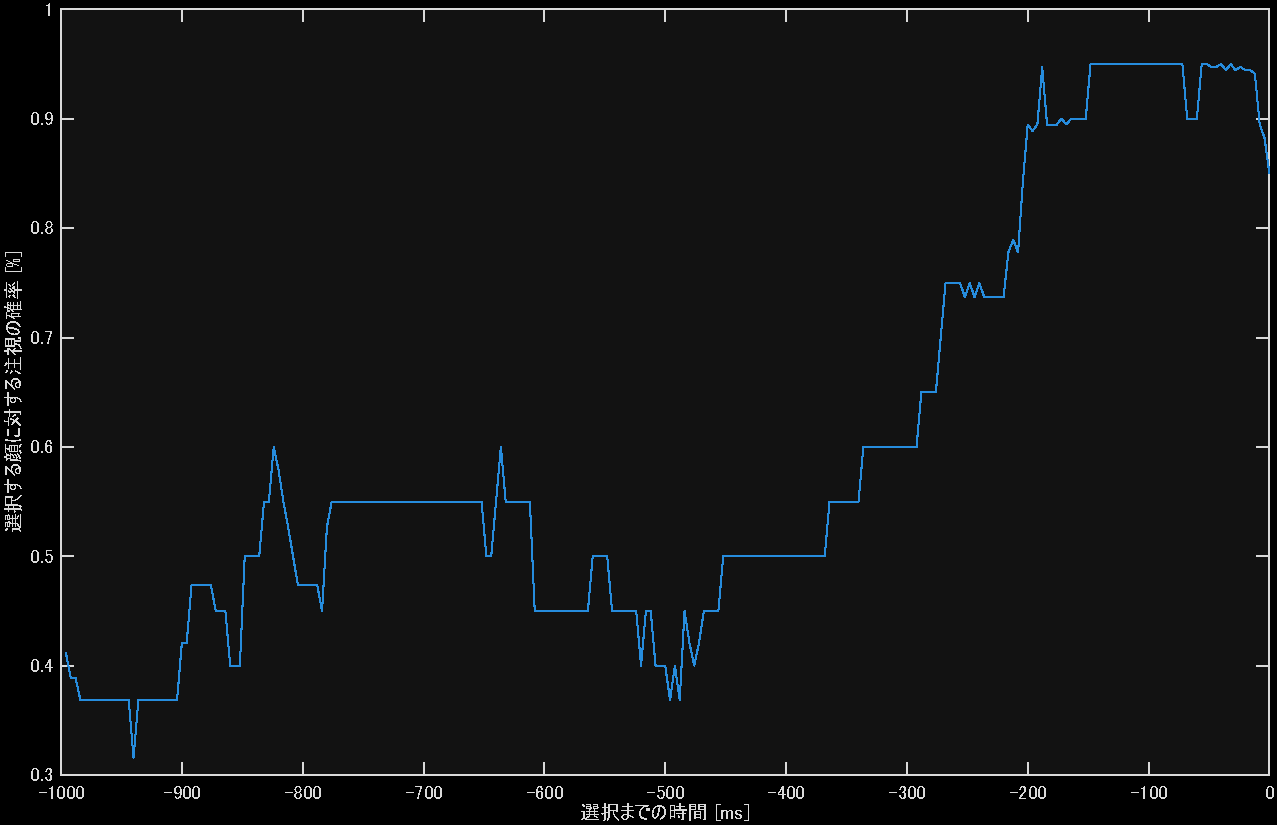
\includegraphics[width=10cm]{exp4_8_2.pdf}
  \caption{選択までの時間と選択する顔に対する注視の確率}
  \label{fig:cascade}
\end{figure}

\subsubsection{考察}
図\ref{fig:cascade}に示されたように，選択の約1秒前から最終的に選択する顔画像に対する注視確率が上昇する視線のカスケード現象が確認された．これは，単に好みの顔だから見るというだけでなく，長く見ることで好みが形成されるという，視線と選好の相互作用を示唆していると考えられる．

\subsection{自由観察時における眼球運動の可視化}
\subsubsection{目的}
対象を自由に見るときの眼球運動を計測し，Gaze PlotおよびHeat Mapとして可視化することで，視線がどのように分布・移動するかを確認することを目的とする．

\subsubsection{方法}
メガネ型眼球運動計測装置（Tobii Glass 3）を使用した\cite{nanoxeed}．実験参加者にアイトラッキング用メガネを装着させ，呈示されるマーカを追視させることで視線方向のキャリブレーションを行った．その後，対象を自由に観察させ，その際の眼球運動を記録した．記録されたデータから，視線の位置や順序を示すGaze Plotおよび，視線の分布を色で示すHeat Mapを作成した．

\section{脳波計測実験（ブレイン・マシン・インタフェース）}
\subsection{目的}
タイプしたい文字を脳情報のみから指定するブレイン・マシン・インタフェース（BMI）のシステムを体験し，事象関連電位（P300）\cite{kango_roo_eeg}を利用した機械学習による判別器の作成とタイピングの原理を学ぶことを目的とする．

\subsection{方法}
脳波計としてg.USBamp（g.tec社）およびドライアクティブ電極を使用し，ソフトウェアとしてMatlabおよびSimulinkを用いた．参加者の頭部にドライ電極を装着し（Fz, Cz, P3, Pz, P4, PO7, Oz, PO8，参照電極は耳たぶ，接地電極は額），サンプリング周波数256Hz，0.1〜30Hzのバンドパスフィルタを適用して脳波を計測した．

被験者はPC上に提示された$6\times6$の文字マトリクスを観察した．ランダムな順で1文字が100msだけ白色に変わり，その後75msは灰色となるフラッシュ刺激が提示された．被験者には特定の文字に集中し，指定された文字が白く変わるたびに回数を数えさせた．トレーニングモードで学習データを測定した後，g.BSanalyzeを用いてターゲット条件と非ターゲット条件の波形パターンを学習させ，線形判別分析（LDA）による判別器を作成した．その後，テストモードで同様のタイピング実験を行った．

\subsection{結果}
脳波計測時の実験風景を図\ref{fig:bmi_device}に，PC上に提示された文字入力用の$6\times6$マトリクス画面を図\ref{fig:bmi_moji}に示す．これらを用いて，事象関連電位P300を指標とした文字入力の体験を行った．

\begin{figure}[htbp]
  \centering
  \begin{minipage}{0.45\columnwidth}
    \centering
    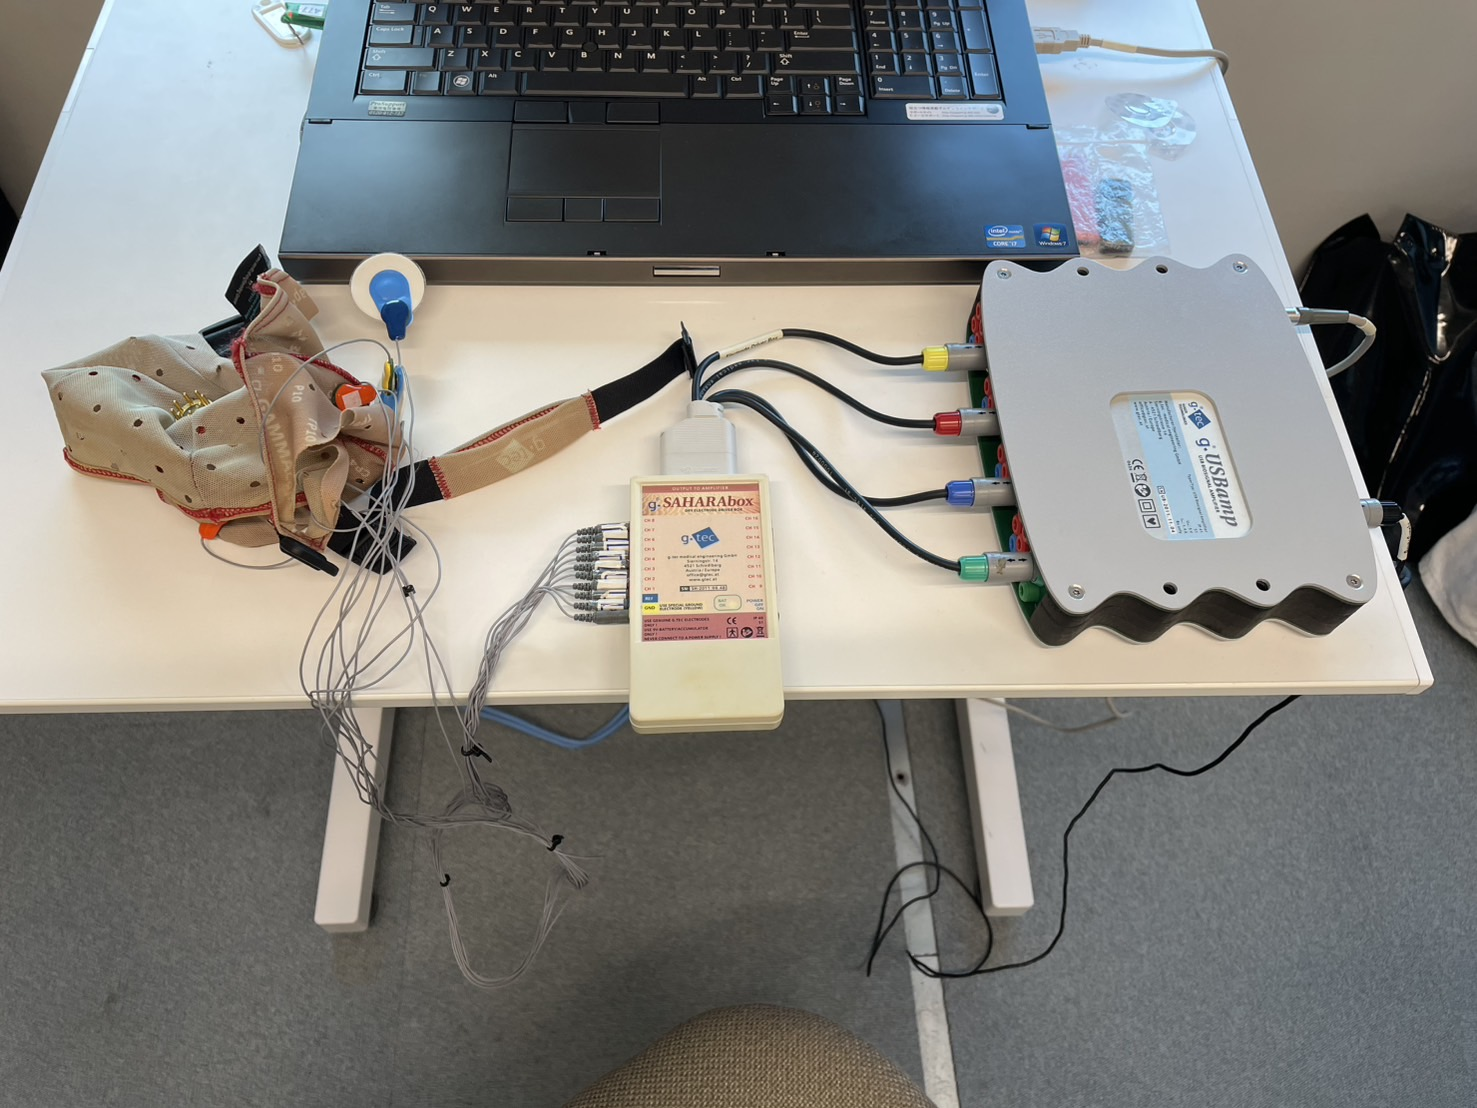
\includegraphics[width=\columnwidth]{moji_device.JPG}
    \caption{BMI実験の様子}
    \label{fig:bmi_device}
  \end{minipage}
  \hspace{0.04\columnwidth}
  \begin{minipage}{0.45\columnwidth}
    \centering
    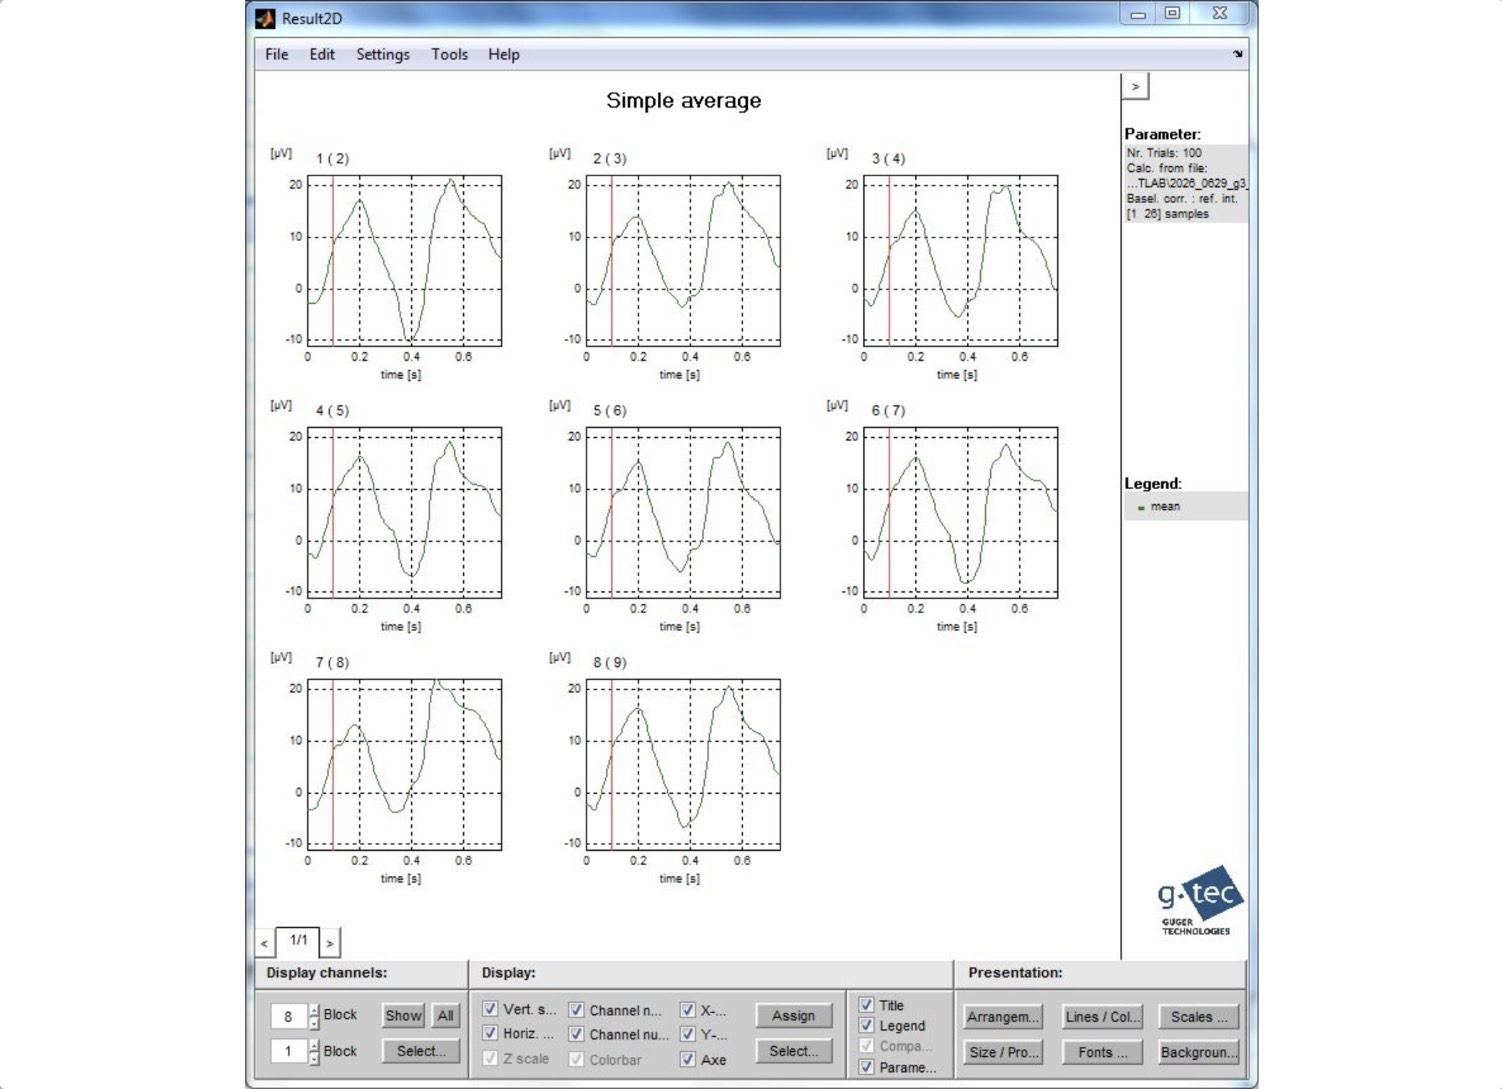
\includegraphics[width=\columnwidth]{moji.JPG}
    \caption{文字入力マトリクス画面}
    \label{fig:bmi_moji}
  \end{minipage}
\end{figure}

\subsection{考察}
事象関連電位であるP300を指標とすることで，被験者がターゲット文字に注意を向けた際に特異的に現れる陽性の電位変動を捉えることができた．この波形パターンを線形判別分析（LDA）によって機械学習させることで，運動出力を伴わずに脳情報のみから意図した文字を指定するBMIの基本的な原理を確認できた．

\section{筋電計測実験}
\subsection{目的}
筋肉が収縮する際に生じる表面筋電図は，発揮する張力や動員される筋線維の数と関連がある\cite{sakaimed_emg}．本実験では，上腕二頭筋を用いて等尺性収縮による最大随意収縮（MVC）および異なる重量のダンベル保持時の筋活動を計測し，発揮張力の増加に伴って表面筋電図の振幅がどのように変化するかを明らかにすることを目的とする．

\subsection{方法}
実験参加者は10班の代表者1名とした．上腕二頭筋の筋活動を計測するための装置として，生体アンプにP-EMG plus（追坂電子機器社），A/D変換器にPowerLab，データの取り込みと解析ソフトウェアにLabChartを使用した．

参加者の上腕二頭筋の筋腹部分に，電極間距離が約2cmとなるように2つの記録電極を貼り付けた．また，接地電極は肩峰に装着した．データのサンプリング周波数は1000Hzに設定した．

計測手順として，まず最大随意収縮（MVC）の計測を行った．参加者に安静状態から腕を90度曲げた姿勢をとらせ，机などの動かない対象物に対して等尺性収縮による最大筋力を発揮させ，その際の筋活動を記録した．次に，参加者が無理なく持ち上げられる異なる重量のダンベルを3種類選択させた．安静状態から1つ目のダンベルを持ち上げ，腕を90度曲げた姿勢で保持している最中の筋活動を計測した．残りの2種類のダンベルについても同様の手順で保持中の筋活動を計測した．

\subsection{結果}
各重量のダンベルを保持した際の上腕二頭筋の表面筋電図について，最大随意収縮（MVC）で正規化した筋活動量の結果を図\ref{fig:emg_result}に示す．図\ref{fig:emg_result}より，保持するダンベルの重量が増加するに伴い，正規化された筋電位の振幅も増加する傾向が確認された．

\begin{figure}[htbp]
  \centering
  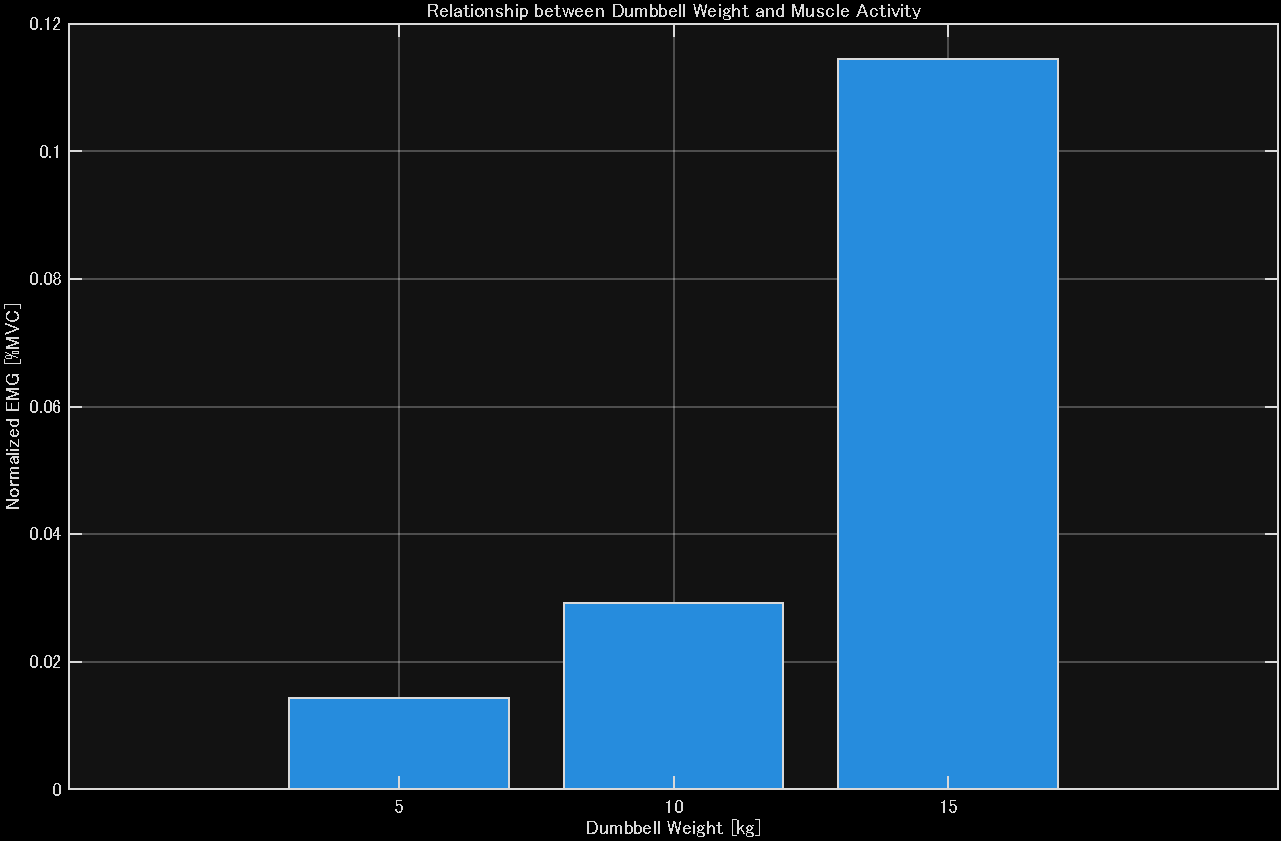
\includegraphics[width=10cm]{exp4_10_7.pdf}
  \caption{ダンベルの重量と正規化された筋活動量}
  \label{fig:emg_result}
\end{figure}

\subsection{考察}
図\ref{fig:emg_result}より，保持するダンベルの重量（負荷）が増加するに伴い，正規化された表面筋電図の振幅が大きくなることが示された．筋肉がより大きな張力を発揮するためには，活動する筋線維（運動単位）の動員数を増やすことや，運動ニューロンの発火頻度を上げることが必要となる．負荷の増大によってこれらが増加した結果，表面から計測される電位の重なりが増え，筋電図の振幅が大きくなったと考えられる．

\begin{thebibliography}{99}
  \bibitem{bsd_eyemovement} 脳科学辞典， ``眼球運動''， https://bsd.neuroinf.jp/wiki/眼球運動
  \bibitem{nanoxeed} 株式会社ナノシード， ``アイトラッキング（視線計測）について''， https://nanoxeed.co.jp/technologyinfo/eyetracking/
  \bibitem{sakaimed_emg} 酒井医療株式会社， ``表面筋電図の臨床応用 その1''， https://www.sakaimed.co.jp/knowledge/surface-electromyogram/clinical/clinical01/
  \bibitem{kango_roo_eeg} 看護roo!， ``脳波の種類''， https://www.kango-roo.com/learning/2159/
  \bibitem{tane_michimata} 田根健吾, 道又爾， ``注視時間の偏りが選好判断に与える影響''， Technical Report on Attention and Cognition, No.13, 2012， https://www.l.u-tokyo.ac.jp/AandC/documents/past/14/13\_TaneMichimata.pdf
\end{thebibliography}

\appendix
\section{プログラムのソースコード}
\subsection{眼球運動計測実験解析プログラム}
\lstinputlisting[language=Matlab]{exp4_8.m}

\subsection{筋電計測実験解析プログラム}
\lstinputlisting[language=Matlab]{exp4_10.m}

\end{document}
